\documentclass[11pt]{article}

\usepackage[utf8]{inputenc}
\usepackage[T1]{fontenc}
\usepackage{amsmath,amssymb}
\usepackage{booktabs}
\usepackage{graphicx}
\usepackage{subcaption}
\usepackage{hyperref}
\usepackage[margin=1in]{geometry}
\usepackage{xcolor}
\graphicspath{{../img/}{../img/paper/}}
\hypersetup{colorlinks=true, linkcolor=blue, citecolor=blue, urlcolor=blue}

\title{\textbf{NeuroSAT: Neuro-symbolic Approaches to the SAT Problem}\\[2mm]
\large Reinforcement learning (Alpha(Go)Zero / DQN) with CNNs and Graph Neural
Networks for SAT-solver branching heuristics}
\author{Donato Meoli}
\date{}

\begin{document}
\maketitle

\begin{abstract}
We study, modernise and extend two neuro-symbolic approaches that learn branching
heuristics for a Boolean SAT solver: (i) an \emph{Alpha(Go)Zero}-style method that
casts SAT solving as a single-player game and combines Monte Carlo Tree Search
(MCTS) with a convolutional policy/value network~\cite{wang2018}; and (ii)
\emph{Graph-Q-SAT}, a value-based reinforcement-learning method that approximates
the $Q$-function over a graph representation of the formula with a Graph Neural
Network (GNN)~\cite{kurin2020}. We introduce \emph{GAT-Q-SAT}, a variant that
injects Graph Attention layers into the message passing. The original
implementations are several years old and depend on TensorFlow~1.x, GSL and
pinned, hard-to-install libraries; we port both to a single, self-contained,
latest-version PyTorch stack, remove the brittle native dependencies, and
\emph{reproduce the original evaluation results exactly}. With clean
attention-on/off ablations at matched training sets, we show that graph attention
is consistently advantageous on \emph{structured} problems (graph colouring) ---
both in-distribution and under transfer, with the advantage \emph{growing with
problem size} --- whereas on uniform-random 3-SAT it provides no benefit and can
hurt. All code, trained runs and figures are reproducible from the repository.
\end{abstract}

\section{Introduction}
Boolean satisfiability (SAT) is the canonical NP-complete problem and underlies
applications in verification, planning and synthesis. Modern solvers are based on
Conflict-Driven Clause Learning (CDCL) and rely on hand-crafted heuristics --- most
notably VSIDS --- to decide which variable to branch on next. The branching
heuristic is a natural target for machine learning: a good policy can prune the
search tree, especially during the ``warm-up'' phase where counter-based
heuristics make poor decisions.

This project implements, \emph{modernises} and \emph{experimentally extends} two
complementary learning approaches, developed in the context of the Pattern
Recognition and Reinforcement Learning courses at the University of Pisa.
Our contributions are:
\begin{enumerate}
  \item A faithful port of both approaches from TensorFlow~1.x (and a GSL-based C++
        MCTS environment) to a single modern PyTorch / PyTorch-Geometric stack, with
        the brittle native dependencies removed.
  \item Exact reproduction of the published Graph-Q-SAT results, used as a
        semantic non-regression oracle for the port.
  \item \textbf{GAT-Q-SAT}, an attention-augmented variant, together with a clean
        experimental study (attention on/off at matched training sets) showing
        \emph{where} and \emph{by how much} attention helps.
\end{enumerate}

\section{Background}
\paragraph{SAT and CDCL.} A CDCL solver repeatedly (i) \emph{decides} a variable
and assigns it a value, (ii) performs unit propagation, and (iii) on a conflict,
\emph{learns} a clause and backtracks. The branching heuristic chooses the
decision variable; replacing or guiding it with a learned policy is the goal here.

\paragraph{Reinforcement learning.} We model the problem as a Markov Decision
Process. Graph-Q-SAT uses DQN to approximate the optimal action-value function
$Q^\star(s,a)=\mathbb{E}[r+\gamma\max_{a'}Q^\star(s',a')]$ with a target network
and experience replay. The Alpha(Go)Zero method instead learns a policy prior
$\pi$ and a value $v$, and uses MCTS to produce improved targets by simulation.

\section{Method 1 --- Alpha(Go)Zero for SAT}
\paragraph{Formulation~\cite{wang2018}.} The CNF formula is represented as a
fixed-size sparse matrix of \emph{clauses} $\times$ \emph{variables}, where an entry
encodes the literal polarity. A convolutional network with a policy head $\pi$
(over the $2\,n_{\text{var}}$ actions ``assign variable true/false'') and a value
head $v\in[-1,1]$ scores states. MiniSat is extended into a game environment that
supports MCTS \emph{simulations}: it returns the would-be state for a sequence of
branching decisions without irreversibly changing the real state. Self-play
collects $(\text{state},\ \text{MCTS visit distribution},\ \text{outcome})$ tuples,
on which the network is trained with the AlphaZero objective
\begin{equation}
  \mathcal{L} = -\textstyle\sum_a \pi^{\text{MCTS}}_a \log \pi_a
              + (z - v)^2 + c\,\lVert\theta\rVert_2^2 .
\end{equation}
A fixed-size CNN cannot generalise across problem sizes; this limitation motivates
the graph-based method below.

\paragraph{Modernisation (this work).} We re-implement the three networks in PyTorch
(\texttt{models\_torch.py}), reproduce the AlphaZero loss and training loop in an
\texttt{AZTrainer} (\texttt{alphazero\_torch.py}), and rewrite the self-play /
supervised-training driver (\texttt{train\_torch.py}). Crucially, we \textbf{remove
the GSL dependency}: the Dirichlet exploration noise is reimplemented with the
C++11 \texttt{<random>} facilities, so the simulation environment builds with
nothing but \texttt{g++} and \texttt{zlib}. The pipeline trains end-to-end on
uniform-random 3-SAT (\texttt{uf20-91}) on both CPU and GPU.

\section{Method 2 --- Graph-Q-SAT and GAT-Q-SAT}
\paragraph{Formulation~\cite{kurin2020}.} The state is a bipartite graph with
variable nodes and clause nodes; node features are 2-D one-hot vectors and edge
features encode literal polarity, with an empty global attribute. There are two
actions per unassigned variable; the agent takes the $\arg\max$ of the $Q$-values
over variable nodes. The reward is a constant $-p$ per non-terminal step and $0$ at
termination. The $Q$-function is an \emph{encode--process--decode} graph
network~\cite{battaglia2018}, trained with DQN. Performance is measured by the
Median Relative Iteration Reduction (MRIR): MiniSat iterations divided by the
model's iterations (values $>1$ mean fewer iterations than MiniSat).

\paragraph{GAT-Q-SAT (this work).} We add an attention pathway to the core graph
block: two edge-aware, multi-head \texttt{GATConv} layers~\cite{velickovic2018}
refine the node embeddings before the global update. Attention lets the model
weight neighbouring clauses/variables, which we hypothesise is beneficial when the
instance has an exploitable sub-structure.

\paragraph{Modernisation (this work).} We port Graph-Q-SAT to the latest
PyTorch / PyTorch-Geometric. We drop the hard-to-install
\texttt{torch-scatter}/\texttt{torch-sparse} (replaced by
\texttt{torch\_geometric.utils.scatter}), make the gym dependency version-robust
(the environment is constructed directly, bypassing the \texttt{gym.make}
env-checker, and works on \texttt{gymnasium}), and add a version-agnostic checkpoint
loader that bridges the \texttt{GATConv} parameter naming across
PyTorch-Geometric versions. The stack uses the latest \texttt{numpy} ($\geq 2$);
the MiniSat gym extension is rebuilt against it.

\paragraph{Exact reproduction.} We verified that the modernised stack does not
change the semantics by re-running the evaluation of the \emph{original trained
checkpoints}: the numbers match the committed logs exactly, e.g.\ on
\texttt{flat30-60} (cap 500) median MRIR $1.833$ (Graph-Q-SAT) and $1.667$
(GAT-Q-SAT), identical to the originals.

\section{Experiments}
\paragraph{Setup.} We use SATLIB instances: uniform-random 3-SAT (\texttt{uf}/\texttt{uuf},
50/100/250 variables, satisfiable / unsatisfiable) and graph colouring
(\texttt{flat}, 30--200 nodes). We cap the number of model decisions before handing
control back to MiniSat at $\{10,50,100,300,500,1000\}$. Crucially, the available
runs form \textbf{clean attention-on/off ablations at matched training sets}:
models trained on graph colouring (\texttt{flat50-115}) and models trained on
random 3-SAT, each with and without attention, averaged over runs. We report MRIR
at cap 500 unless noted.

\paragraph{Main result.} Figure~\ref{fig:thesis} summarises the central finding.
\begin{figure}[h]
\centering
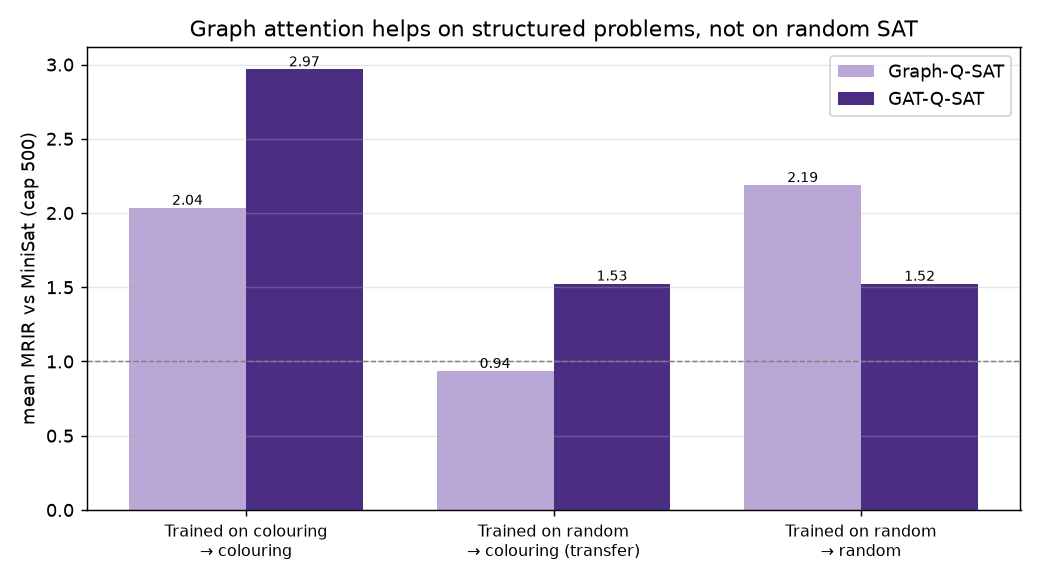
\includegraphics[width=0.82\textwidth]{thesis.png}
\caption{Mean MRIR vs MiniSat (cap 500) per regime. Graph attention (GAT-Q-SAT)
clearly helps on graph colouring --- both in-distribution and under transfer from
random training, where plain Graph-Q-SAT even drops \emph{below} $1$ (slower than
MiniSat). On uniform-random 3-SAT, attention provides no benefit.}
\label{fig:thesis}
\end{figure}

\paragraph{(1) In-distribution graph colouring.} Trained and tested on graph
colouring, GAT-Q-SAT beats Graph-Q-SAT on \emph{every} size, and the gap
\textbf{grows with problem size}: plain Graph-Q-SAT degrades on the largest
instances (\texttt{flat200-479}: $1.35$) while GAT-Q-SAT holds up ($3.39$), a
$+2.04$ MRIR gap. This is the regime where attention pays off most.

\paragraph{(2) Transfer (random $\to$ colouring).} Trained only on random 3-SAT and
evaluated on graph colouring, Graph-Q-SAT frequently falls \emph{below} $1$
(\,$0.78$--$0.97$, i.e.\ worse than MiniSat), whereas GAT-Q-SAT stays above $1$
($1.16$--$1.75$) on all sizes. Attention substantially improves zero-shot transfer
to structured problems (Fig.~\ref{fig:curves}, middle).

\paragraph{(3) Uniform-random 3-SAT.} Here attention does \emph{not} help and can
hurt: on \texttt{uf250-1065}, plain Graph-Q-SAT reaches $4.78$ against GAT-Q-SAT's
$1.69$. Random formulas near the phase transition lack the structure attention can
exploit.

\begin{figure}[h]
\centering
\begin{subfigure}{0.33\textwidth}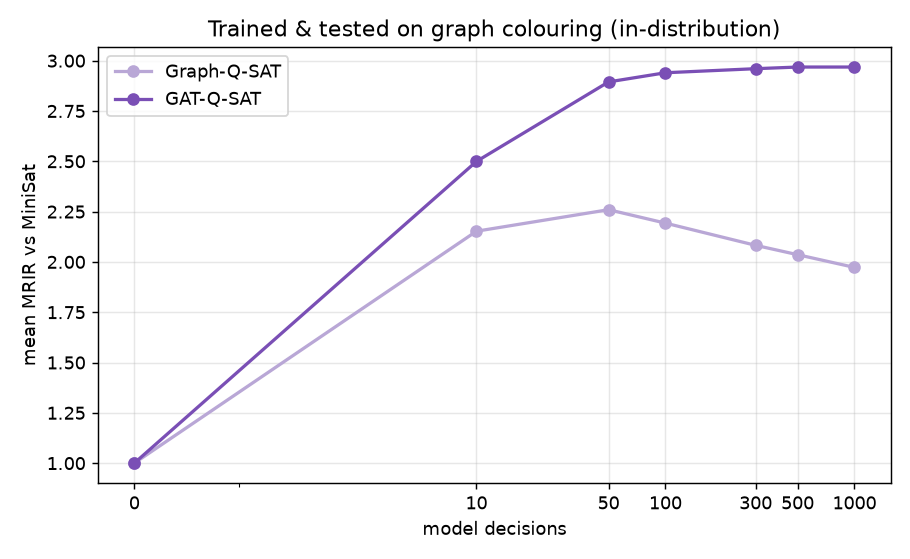
\includegraphics[width=\textwidth]{coloring_indist.png}\end{subfigure}
\begin{subfigure}{0.33\textwidth}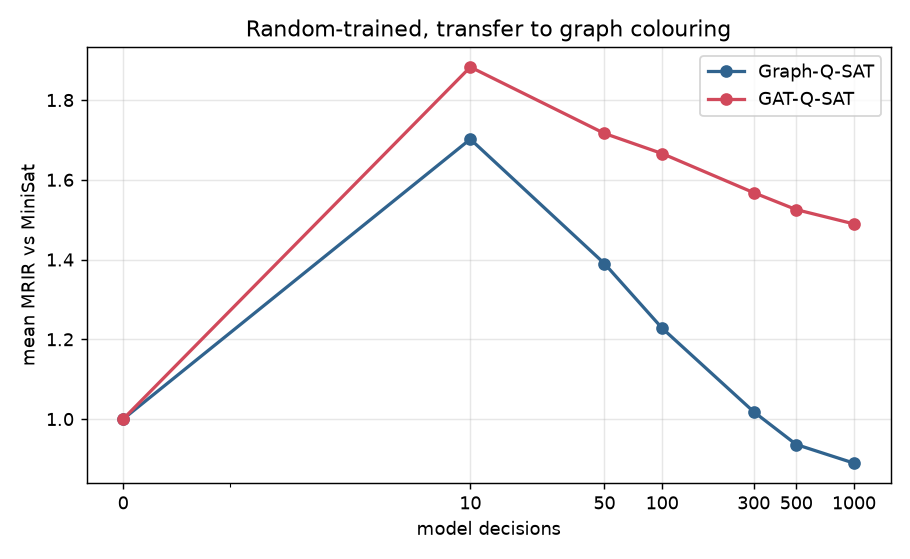
\includegraphics[width=\textwidth]{random_transfer.png}\end{subfigure}
\begin{subfigure}{0.33\textwidth}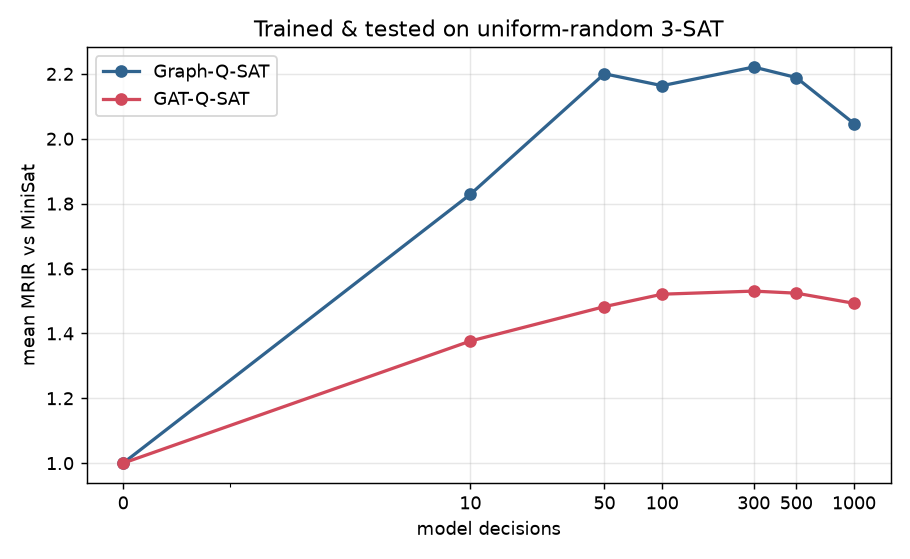
\includegraphics[width=\textwidth]{random_indist.png}\end{subfigure}
\caption{MRIR vs the number of model decisions. Left: trained and tested on graph
colouring. Middle: random-trained, transferred to colouring. Right: trained and
tested on random 3-SAT. Attention helps in the first two (structured) settings and
not in the third.}
\label{fig:curves}
\end{figure}

\paragraph{Generalisation across size.} Figure~\ref{fig:gen} plots MRIR against the
number of variables for the random-trained models. On graph colouring the
attention model's advantage is stable and pronounced across sizes; on random
instances the ordering is reversed.
\begin{figure}[h]
\centering
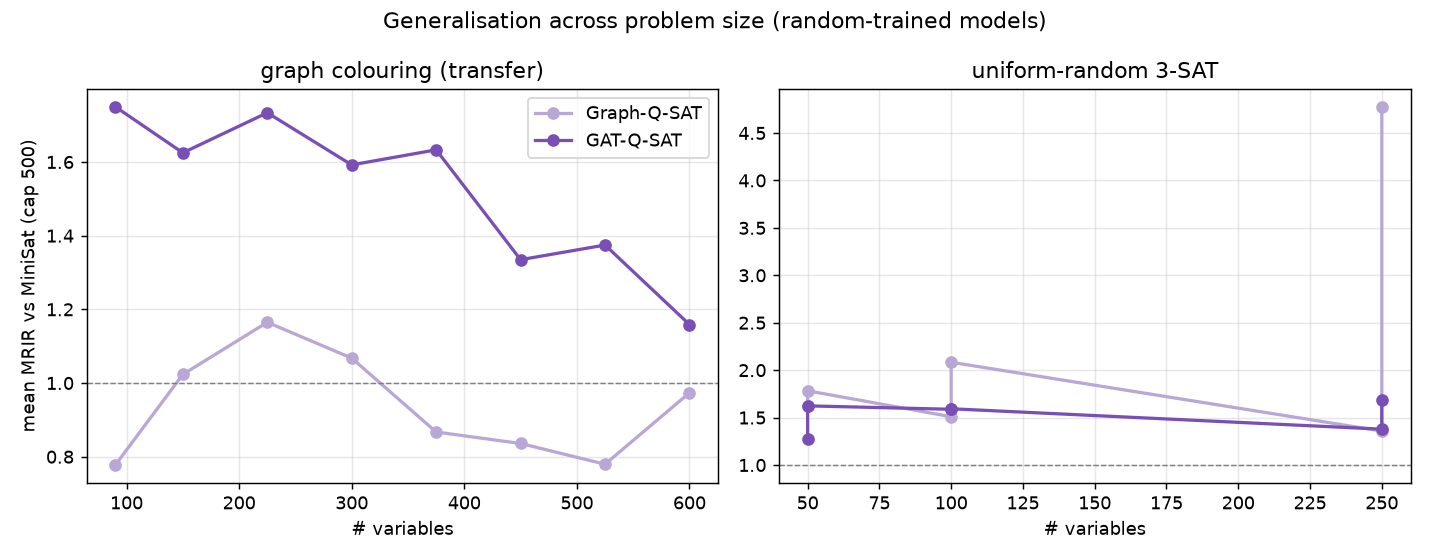
\includegraphics[width=0.92\textwidth]{generalization.png}
\caption{Generalisation across problem size (random-trained models, cap 500).}
\label{fig:gen}
\end{figure}

\paragraph{Per-size numbers.} Table~\ref{tab:numbers} gives the in-distribution
graph-colouring MRIR per size, making the size-growing attention advantage explicit.
\begin{table}[h]\centering\small
\begin{tabular}{lccc}
\toprule
graph-colouring set & Graph-Q-SAT & GAT-Q-SAT & $\Delta$ \\
\midrule
flat30-60   & 1.83 & 2.00 & $+0.17$ \\
flat75-180  & 2.37 & 2.94 & $+0.58$ \\
flat125-301 & 2.55 & 3.44 & $+0.88$ \\
flat150-360 & 1.92 & 3.76 & $+1.85$ \\
flat200-479 & 1.35 & 3.39 & $+2.04$ \\
\bottomrule
\end{tabular}
\caption{In-distribution graph colouring, mean MRIR at cap 500. The attention
advantage grows with problem size.}
\label{tab:numbers}
\end{table}

\paragraph{Reproducibility.} All figures and tables are regenerated from the
evaluation logs (\texttt{GQSAT/runs/*/*.tsv}) by \texttt{aggregate\_results.py},
\texttt{make\_plots.py} and \texttt{paper\_analysis.py} --- no manual spreadsheets.
Training is reproducible on a Colab GPU via \texttt{notebooks/train\_colab.ipynb}
(checkpointing to Drive with automatic resume).

\section{Related Work}
The field has converged on graph- and attention-based models for SAT. NeuroSAT
learns satisfiability from single-bit supervision~\cite{neurosat}; NeuroCore
predicts unsat-core variables to refine branching~\cite{neurocore}; NeuroComb and
\textbf{NeuroBack}~\cite{neuroback} move inference \emph{offline} (a single query
before solving) and, using a Graph Transformer with self-attention, achieve the
first wall-clock speed-ups on industrial instances (Kissat, SAT Competition). This
trajectory is notable for two reasons relevant to this project: (i) the move to
\emph{attention} on SAT graphs corroborates the GAT-Q-SAT direction; and (ii) the
known limitation of Graph-Q-SAT --- online inference is too slow for wall-clock
gains --- is exactly what offline, one-shot inference overcomes. Recent work
continues along the RL-from-algorithm-feedback and restricted-heuristics
lines~\cite{mlforsat2023}, and surveys catalogue the design space~\cite{survey2025}.

\section{Conclusions}
We modernised two neuro-symbolic SAT methods to one self-contained, latest-version
PyTorch stack, removed their brittle native dependencies (TensorFlow~1.x, GSL,
\texttt{torch-scatter}/\texttt{torch-sparse}, pinned gym), and reproduced the
original results exactly. With clean attention-on/off ablations we established a
crisp, size-dependent result: \textbf{graph attention helps on structured problems
(graph colouring), in-distribution and under transfer, with the advantage growing
with problem size, while it does not help on uniform-random 3-SAT}. The fixed-size
CNN of the Alpha(Go)Zero method, while elegant, cannot generalise across sizes ---
the gap that graph methods, and the subsequent literature (NeuroCore/Comb/Back),
were designed to close. Promising next steps are larger attention/Graph-Transformer
back-ends and offline inference for genuine wall-clock gains.

\begin{thebibliography}{9}
\bibitem{wang2018} F. Wang and T. Rompf. \emph{From Gameplay to Symbolic Reasoning:
  Learning SAT Solver Heuristics in the Style of Alpha(Go) Zero}. arXiv:1802.05340, 2018.
\bibitem{kurin2020} V. Kurin, S. Godil, S. Whiteson, B. Catanzaro. \emph{Can
  Q-Learning with Graph Networks Learn a Generalizable Branching Heuristic for a
  SAT Solver?} NeurIPS 2020. arXiv:1909.11830.
\bibitem{velickovic2018} P. Veli\v{c}kovi\'c et al. \emph{Graph Attention
  Networks}. ICLR 2018. arXiv:1710.10903.
\bibitem{battaglia2018} P. Battaglia et al. \emph{Relational inductive biases, deep
  learning, and graph networks}. arXiv:1806.01261.
\bibitem{neurosat} D. Selsam et al. \emph{Learning a SAT Solver from Single-Bit
  Supervision}. arXiv:1802.03685.
\bibitem{neurocore} D. Selsam and N. Bj{\o}rner. \emph{Guiding High-Performance SAT
  Solvers with Unsat-Core Predictions}. arXiv:1903.04671.
\bibitem{neuroback} W. Wang et al. \emph{NeuroBack: Improving CDCL SAT Solving using
  Graph Neural Networks}. ICLR 2024. arXiv:2110.14053.
\bibitem{mlforsat2023} \emph{Machine Learning for SAT: Restricted Heuristics and New
  Graph Representations}. arXiv:2307.09141, 2023.
\bibitem{survey2025} \emph{Neural Approaches to SAT Solving: Design Choices and
  Interpretability}. arXiv:2504.01173, 2025.
\end{thebibliography}

\end{document}
